\documentclass[a4paper]{article}

\usepackage[english]{babel}
\usepackage[utf8x]{inputenc}
\usepackage{amsmath}
\usepackage{graphicx}
\usepackage[colorinlistoftodos]{todonotes}
\usepackage{parskip}
\usepackage{float}
\usepackage{hyperref}
\usepackage{fullpage}

\begin{document}

\title{Assignment 2 \\ Secure Data Management}
\author{Rick van Galen - s0167746 (UT) \\ Erwin Middelesch - s0197106 (UT) \\ Jeroen Senden - s0191213 (UT) \\ Bas Stottelaar - s0199141 (UT)}
\date{\today}
\maketitle

\section{Introduction}
	In this repot we will discuss our prototype implementation of assignment 2. The goal of this assignment is to implement a searchable and encrypted transaction system where the storage server, a honest but curious one, should not be able to learn anything. This implementation is based on the work of Hacig{\"u}m{\"u}{\c{s}} et al. \cite{hacigumucs2002executing}.
	
	The implementation is realized with a Python backend and JavaScript for the frontend, to make sure the sensitive keys stay local.
	
	In the first part of this document, we describe the data model. Then the key distribution and implementation. The main part will be about the bucket mapping, querying and searching. We conclude with a discussion.

\section{Data model}
	This section we discuss the database and the frameworks utilized in implementing the system.
    
    \subsection{Database}
    	The database contains three tables created by the system (the rest of the tables are automatically generated by Django, explained in section \ref{sec:frameworks}. These three tables are shown below, together with the field contained in the table and an explanation what the field represents.
        
    \textbf{Client}
    \begin{itemize}
        \item \textbf{Id} - a unique ID for the client.
        \item \textbf{Name} - the name of the client.
        \item \textbf{\{$|$symmetric\_key$|$\}pk$_{consultant}$} - the symmetric key used to encrypt transaction, encrypted with the public key of the chosen consultant (the consultant's ID is also stored in this record). 
        \item \textbf{user\_id} - to link the user to Django's authentication facilities.
        \item \textbf{Client bucket} - the bucket in which the client is placed, such that when a transaction is searched for without criteria, the server won't know that every transaction belongs to this user.
        \item \textbf{Consultant\_id} - the ID of the consultant.
    \end{itemize}
    
    \textbf{Consultant}
    \begin{itemize}
        \item \textbf{Id} - a unique ID for the consultant.
        \item \textbf{Name} - the name of the consultant.
        \item \textbf{public\_exp} - component of the consultant's public key: the exponent $e$ used in the RSA calculation.
        \item \textbf{public\_mod} - component of the consultant's public key: the modulus $n$ used in the RSA calculation.
        \item \textbf{user\_id} - to link the user to Django's authentication system.
    \end{itemize}
    
    \textbf{Transaction}
    \begin{itemize}
        \item \textbf{Id} - a unique transaction ID
        \item \textbf{Encrypted data \{sender, receiver, amount, description, date\}}, the secret data that only the client and the consultant must be able to decrypt.
        \item \textbf{Amount Bucket} - the bucket that is searchable by everyone (explained in section \ref{sec:bucketamount}).
        \item \textbf{Date bucket} - the bucket that is searchable by everyone (explained in section \ref{sec:bucketdate}).
        \item \textbf{Client bucket} - the bucket that states to which clients this transaction belongs in order to minimize the results and thus minimize the overhead of sending transactions which the client and consultant will not be able to decrypt (explained in section \ref{sec:bucketclient}). 
    \end{itemize}
    
    \subsection{Used libaries \& frameworks} \label{sec:frameworks}
    \begin{description}
    	\item[Django\footnotemark]
        	\footnotetext{\url{https://www.djangoproject.com/}}
        	Django is a web application framework to write server side web applications in Python. Django is used in this project to serve the project files, provide authentication features and to perform translation of the JavaScript data structures to the database layer.
        
        \item[Angular.js\footnotemark]
        	\footnotetext{\url{https://angularjs.org}}
        	Angular.js is a framework to write dynamic web applications that run almost entirely in web browsers. Since the browser based client performs most of the business logic in our application, we decided to use this framework to also perform most of the web application logic. For this, Angular performs routing, dynamic template rendering and separation of concerns.
            
        \item[Bootstrap\footnotemark]
        	\footnotetext{\url{https://getbootstrap.com}}
			Bootstrap is a CSS framework developed by Twitter. It provides a uniform and well-designed styles for creating web applications. The use of Bootstrap improves the user experience of our system.
        
        \item[CryptoJS\footnotemark and rsa.js\footnotemark]
        \footnotetext{\url{https://code.google.com/p/crypto-js/}}
        \footnotetext{\url{http://www-cs-students.stanford.edu/~tjw/jsbn/}}
        Cryptography in JavaScript is provided by two libraries. CryptoJS is a library that implements commonly needed cryptographic constructs, and is used in our application to provide the AES-cipher as well as the SHA3-512 cryptographic hash function. To implement support for public-key infrastructure with the RSA crypto system we used Tom Wu's \texttt{rsa.js} library developed at Stanford University.
    \end{description}
            
            
\section{Key distribution scheme}

There are multiple ways to distribute the keys. We chose to use shared symmetric keys between the consultant and a client. The client generates a key based on his username and password when he registers to the system and chooses his consultant. In order to make it space efficient for the consultant (i.e. so that he does not need to remember every symmetric key with every client), we chose to store the symmetric key on the server. To store this key in such a way that the server cannot use this key, the consultant has a private-public key pair. The symmetric key is stored on the server, encrypted with the public key of the consultant. To retrieve the symmetric key used to decrypt the transactions, the consultant will first need to decrypt the symmetric key with his private key.  By doing it this way, both parties only need to remember one key. The client remembers his chosen username and password, and the consultant only needs to remember his secret key. 

To make the system easier to use for clients, we decided to use the same username and password to authenticate the user with the system as well as passphrase used for the symmetric encryption. To prevent both client and server from learning the plaintext of this password, the password is hashed in different ways for both cases. For the server, we perform client side hashing function by applying the SHA3 algorithm to the plaintext password before it is submitted for registration. In our implementation, the server in turn hashes this string using the PBKDF2 hashing and salting algorithm before storing it. For the symmetric key, the SHA3 hashing function is applied to the plaintext password \emph{concatenated} to the user's username. When the consultant decrypts the stored symmetric key, he will see the hashed text and not the plaintext password. No information about the user's password will be revealed even if the consultant and the server collude. A schematic representation of the key distribution is shown in figure \ref{fig:keydist}. Since both the consultant and client share the same hashed key, it can be used as input for the symmetric AES256 cipher to encrypt and decrypt transaction data.

\begin{figure}
\centering
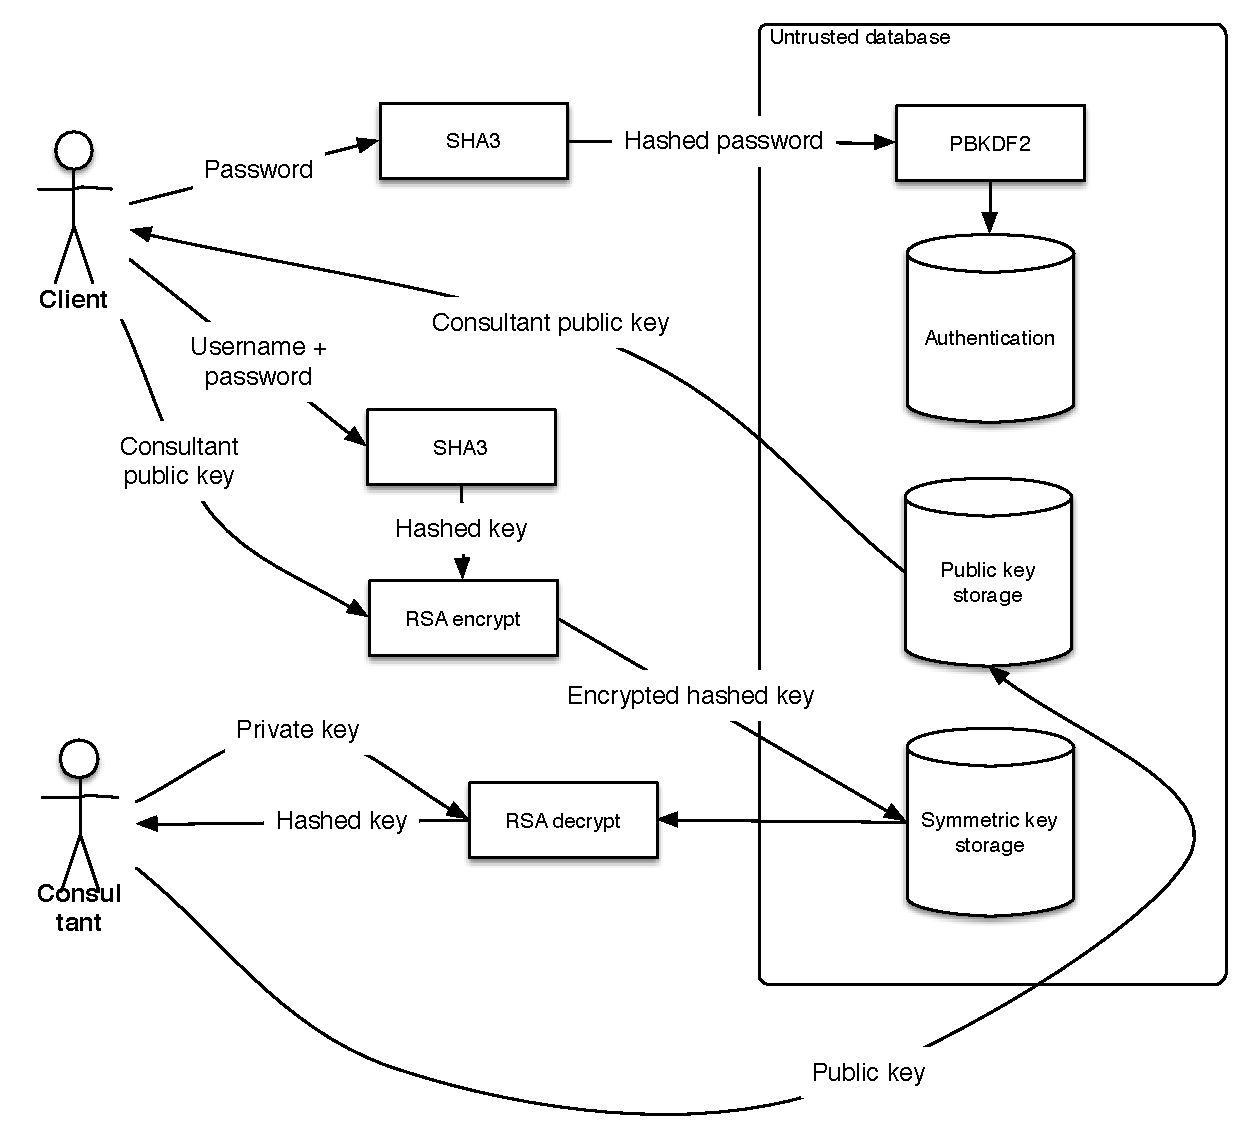
\includegraphics[scale=0.5]{keydist.pdf}
\caption{The key distribution scheme. Because both client and consultant can access the hashed key it can be used for symmetric encryption.}
\label{fig:keydist}
\end{figure}

\section{Mapping scheme}
	The current mapping scheme is just a basic example of how a mapping scheme should look like. Table \ref{tab:amountbucket} shows the mapping scheme for amount. Table \ref{tab:datebucket} shows the mapping scheme for the date. 
    
\subsection{Bucket algorithms}
	The pseudocode below describes the algorithms used to determine the bucket value of a single transaction, or a list of bucket values based on an upper and lower value. Only the functions for the field amount are given, the functions for date are similar.

\begin{verbatim}
amount_bucket_map = [] #1

function generateAmountQuery(lower_amount, upper_amount){ #2
   lower_index = amountToIndex(lower_amount)
   upper_index = amountToIndex(upper_amount)
   
   return indexToBucketValues(lower_index, upper_index, amount_bucket_map.length/2, "amount") #3
}

function amountToIndex(amount) { #4
    index = amount_bucket_map.length -1
    for (int i = 0; i < amount_bucket_map.length -1; i++){
        if amount_bucket_map[i] <= amount && amount < amount_bucket_map[i+1] {
            index = i
            break
        }
    }
    return index
}
    
function indexToBucketValues(lower_index, upper_index, number_of_buckets, field) {
    values = []
    for (int i = lower_index; i < upper_index + 1; i++){
        values.add(indexToBucketValue(i%number_of_buckets,field) #5
    }        
    values.sort() #6
    values.deleteDuplicates() #7
    return values.join(',')
}
     
function indexToBucketValue(index, field){ #8
    result = SHA-3(index + field + symmetric_key) #9
    return result[0] #10
}
    
\end{verbatim}


\begin{enumerate}
	\item This list contains the table shown in \ref{tab:amountbucket}
    \item This function is called when a user searches for a amount range. It returns for example '1,9,f'
    \item Calls the indexToBucketValues with the lower index, upper index calculated above. And with the number of distinct buckets, as this differs between date and amount. The string "amount" is passed as well to ensure date and amount map to different values.
    \item Calculates the index of a specific amount in the amount\_bucket\_map.
    \item Adds for each index the corresponding bucket value to the list. 
    \item Sorts the list so the server cannot deduce which buckets correspond to high amounts and which buckets correspond with low amounts.
    \item Duplicates have to be deleted because multiple intervals are mapped to the same bucket value.
    \item Returns the bucket value for a certain index and field.
    \item The bucket value is based on the index, field and symmetric key. The field is used to ensure the bucket values for date and amount differ. The symmetric key is used to ensure the server does not know which bucket value corresponds to which range of input values.
    \item The function returns the first character of the hash. The hash is hexadecimal encoded, so there are 16 different possible bucket values. This ensures the odds of 2 buckets mapping to the same value is relatively small, while not having enough distinct values to reliably recognize which client belongs to a transaction based on the bucket value. This also prevents the search-url from exploding when all the buckets need to be searched and keeps the search-url small. Although the HTTP-standard does not state a limit for the length of the url, some webbrowsers and servers might run into difficulties when they receive a url that is too long to handle.  
\end{enumerate}
    
    \subsection{The bucket values}\label{sec:bucket}
    	
        \subsubsection{The amount bucket}\label{sec:bucketamount}
        
        The amount bucket values are based on a normal distribution as given to the following formula:
        
        $y=\int_{-\infty}^x \frac{1}{{\sigma \sqrt {2\pi } }}e^{{{ - \left( {x - \mu } \right)^2 } \mathord{\left/ {\vphantom {{ - \left( {x - \mu } \right)^2 } {2\sigma ^2 }}} \right. \kern-\nulldelimiterspace} {2\sigma ^2 }}}$ 
        
        where $\mu = 5000$ and $\sigma = 2000$. By using these buckets, the server cannot determine in a statistic manner, whether a bucket is for e.g. 5000, because that bucket has more entries then all of the other buckets. Furthermore, by choosing the buckets according to this distribution, a more efficient storing of all the values is achieved. If the server has to look for the bucket where 5200 is in (in our case this results to 5001-5251), the amount of transactions in this buckets is less then when you did a normal mapping of 0-5000 and 5000-10000 etcetera. This is only true if the $\mu$ and $\sigma$ are based on some actual facts. For now, the $\mu$ and $\sigma$ are based on estimations about which values are likely for transaction amounts. In the real world, this $\mu$ and $\sigma$ might be changed to better fit the actual circumstances and get more secure and efficient buckets. The mapping used for now can be found in table \ref{tab:amountbucket}. The first character of the hash is used as the bucket value.
        
        The hash for bucket 0 to 9 is repeated for bucket 10-19 to counter the problem that the server might learn ordering from the queries. Because it is only possible to search for transactions within an interval, the server knows bucket values are consecutive after an user performs a search. As the bucket values are alphabetized the server does not know the ordering. This information can be deduced however. For example, when an user performs a search for bucket values 1,2,5,8,9 and performs another search for bucket values 2,4,6,8,f, information about the ordering of the bucket values can be deduced by the server. Because the bucket values are consecutive, and the two queries have two bucket values in common, 2 and 8, these two bucket values must be consecutive. If an user performs enough searches, the server will know the ordering of all bucket values. This allows the server to estimate the amount of a transaction for some transactions. Because the server knows the ordering, but does not know which bucket value contains the smallest amounts and which contains the largest, it is not possible to deduce the approximate amount for each transaction, but only for the bucket values near the middle of the ordering. It is also possible to approximate the difference between transactions. Therefore we map the second half of the amounts on the same bucket values as the first half. This ensures there is no way to tell the approximate difference in amount between two transactions. The ordering can still be deduced, but it is no longer possible to deduce the lowest and highest bucket values. Therefore it is not possible to estimate the amount of a transaction.
        
        
        
        
        
        \begin{table}[t!]
        \begin{tabular}{| l | l | l |} \hline
            \textbf{Amount} & \textbf{Bucket} & \textbf{hash(bucket)} \\ \hline
            0-1710 & 0 & hash(0 + symmetric key) \\ \hline
            1711-2436 & 1 & hash(1 + symmetric key) \\ \hline
            2437-2927 & 2 & hash(2 + symmetric key) \\ \hline
            2928-3316 & 3 & hash(3 + symmetric key) \\ \hline
            3317-3651 & 4 & hash(4 + symmetric key) \\ \hline
            3652-3951 & 5 & hash(5 + symmetric key) \\ \hline
            3952-4229 & 6 & hash(6 + symmetric key) \\ \hline
            4230-4493 & 7 & hash(7 + symmetric key) \\ \hline
            4494-4748 & 8 & hash(8 + symmetric key) \\ \hline
            4749-5000 & 9 & hash(9 + symmetric key) \\ \hline
            5001-5251 & 10 & hash(0 + symmetric key) \\ \hline
            5252-5506 & 11 & hash(1 + symmetric key) \\ \hline
            5507-5770 & 12 & hash(2 + symmetric key) \\ \hline
            5771-6048 & 13 & hash(3 + symmetric key) \\ \hline
            6049-6348 & 14 & hash(4 + symmetric key) \\ \hline
            6349-6683 & 15 & hash(5 + symmetric key) \\ \hline
            6684-7072 & 16 & hash(6 + symmetric key) \\ \hline
            7073-7563 & 17 & hash(7 + symmetric key) \\ \hline
            7564-8289 & 18 & hash(8 + symmetric key) \\ \hline
            8290-$\infty$ & 19 & hash(9 + symmetric key) \\ \hline
        \end{tabular}
        \caption{The mapping used for amount}\label{tab:amountbucket}
        \end{table}
        
        \subsubsection{The date bucket}\label{sec:bucketdate}
        
        The dates buckets are based on the order of the months in which these dates occur, as shown in table \ref{tab:datebucket}. This means that the bucket value does not care about the day or the year the transaction was done. The server will already know which bucket belongs to which month, since the server knows when the transaction was added into his database and into which bucket. We therefore do not hide the month of the transaction, but we do hide the day that the transaction took place, since this could have been any day of the month, and does not necessarily need to be the day of the upload. Note that in table \ref{tab:datebucket}, the hash for bucket 0 to 5 is repeated for bucket 6-11 to counter the problem that the server might learn ordering from the queries, as explained above. 
        
        \begin{table}[b!]
        \begin{tabular}{| l | l | l |} \hline
            \textbf{Month} & \textbf{Bucket} & \textbf{hash(bucket)} \\ \hline
            January & 0 & hash(0 + symmetric key) \\ \hline
            February & 1 & hash(1 + symmetric key) \\ \hline
            March & 2 & hash(2 + symmetric key) \\ \hline
            April & 3 & hash(3 + symmetric key) \\ \hline
            May & 4 & hash(4 + symmetric key) \\ \hline
            June & 5 & hash(5 + symmetric key) \\ \hline
            July & 6 & hash(0 + symmetric key) \\ \hline
            August & 7 & hash(1 + symmetric key) \\ \hline
            September & 8 & hash(2 + symmetric key) \\ \hline
            October & 9 & hash(3 + symmetric key) \\ \hline
            November & 10 & hash(4 + symmetric key) \\ \hline
            December & 11 & hash(5 + symmetric key) \\ \hline
        \end{tabular}
        \caption{The mapping used for date}\label{tab:datebucket}
        \end{table}
      
      \subsubsection{The client bucket}\label{sec:bucketclient}
           
      Transactions are not directly linked to a client, but are given a client bucket value. This makes it more difficult for the server to determine which client a specific transaction belongs to. Client buckets are assigned when a client registers. Every three consecutive clients share the same bucket value.
      
\section{The query}

	There occur multiple queries to our database in our system. These are: 
    
    \begin{itemize}
    	\item When the user registers to our system
        \item When the user logs in
        \item When the user creates a new transaction
        \item When the user edits his transaction
        \item When the user searches for specific transactions 
    \end{itemize}
    
    The registering and the logging in of the user is handled by Django in our system. We do however have our own table in the database (search\_client and search\_consultant) to have some additional information about the user which we can store (like the client\_bucket that is linked to the client\_bucket of every transaction and the public\_key of the consultant. 
    
    The query that is done when the user creates a new transaction is simply an insert into query, and the editing of a transaction is an update query. Both are handled smoothly by the Django environment.
    
    The search query is the most interesting query, since this is where we search in the encrypted data in the database. We give the buckets in which buckets the server needs to search, and Django fills in the where-clause of the query and gives us back the corresponding transactions. Django knows who logged into the system (i.e. knows his client ID) and can thus also filter the results based on his client\_bucket. In order to let Django know what to put in the where-clause of the query, we send this data in a query. The query is of the form: \verb;/?amount=1,2,f&date=2,d;. When there is no amount specified, the url becomes \verb;/?date=2,d; and when there is no date specified, the url becomes \verb;/?amount=1,2,f; In these examples, the 1,2,f and 2,d are the first character of the mapped value of the amount and date. We are searching for 3 amount-buckets and 2 date-buckets in this example, which means we can search based on $<$, =, $>$, and $><$ operations. We can also search for multiple month buckets, thus 'before' a certain date, 'after' a certain date, 'on' a certain date and 'between' certain dates. 

\section{Decryption}
	When the search query has executed, it returns the encrypted tuple with all the transaction data. Before we can determine whether this result is of the client and whether it satisfies the actual search criteria, we need to decrypt it. This is done by the symmetric key that the client chose at the registration at our system. If the consultant wants to decrypt the data, he simply looks up the symmetric key in the client entry in the client table. This key is encrypted with the public key of the consultant and thus only the consultant can retrieve the symmetric key from this entry. Once the consultant has decrypted the symmetric key, he can decrypt the data tuples that he retrieved from the server. 
	We do however note that the user will also receive some transactions that are not meant for him, i.e. belong to another user. This is because we are currently filtering on the server based on client buckets in order to see whether a transaction belongs to that user. However, there are multiple clients in a client bucket. This is not a problem, since the user won't be able to decrypt the data of the other users since the user does not possess the corresponding symmetric key.   
    
\section{Filtering}
	The system has two filtering systems. Since some results might not belong to the user that executed the query, we need to do some filtering. Since the user does not have the correct symmetric key, he will decrypt gibberish out of the transactions. The decryption algorithm will notice this and will thus discard the transaction. The second filtering is done after the first filter. Since the search criteria are based on buckets, the user might retrieve results that are not what he initially searched for. For example, when the user searches for amounts less then 5200, he will also receive amounts up to 5251, since they are also part of that bucket. Thus, after decryption of the tuples, we need to filter these results out. The transactions that are left after the filtering will be displayed.
    
   	A schematic representation of querying in the encrypted data is given in figure \ref{fig:queries}.
    \begin{figure}
    \centering
    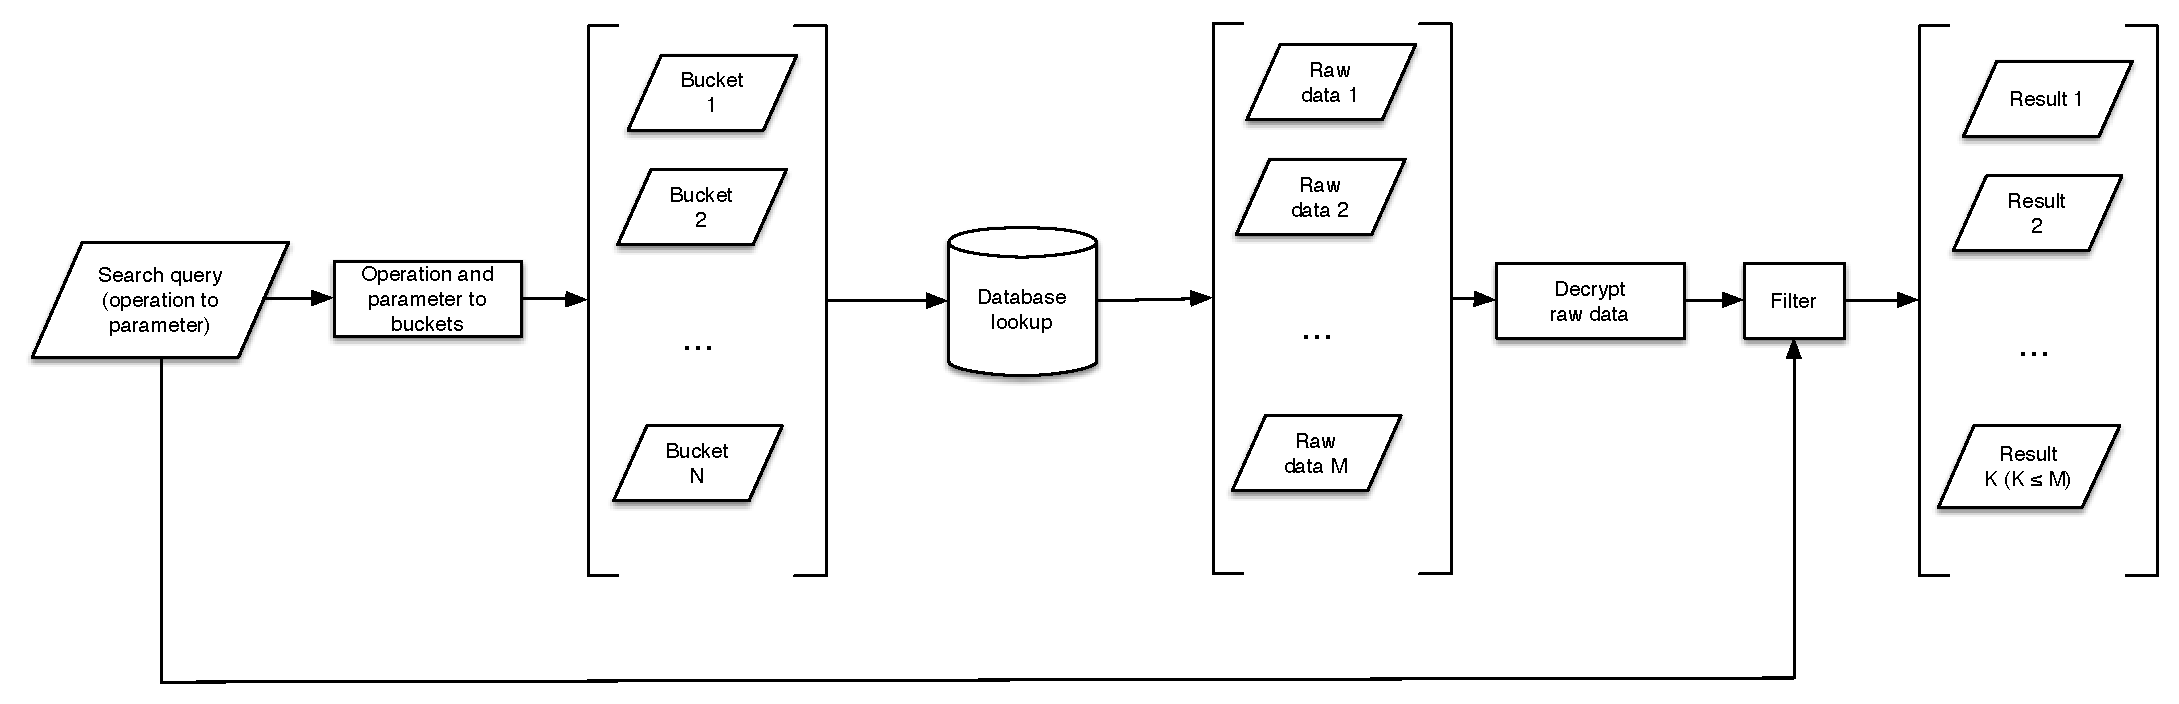
\includegraphics[scale=0.4]{queries.pdf}
    \caption{An overview of bucket based querying}
    \label{fig:queries}
    \end{figure}

\section{Requirement verification}
	There were several requirements that the system had to fulfill. These are stated below. 
	\begin{description}
    	\item[1. The consultant can insert financial data for all of his clients in the storage server.] This requirement is satisfied by the fact that the consultant can look up the encrypted symmetric key in the database with and decrypt it with his private key. Thus only clients that encrypt their symmetric key with the public key of the consultant give that consultant access to their data. 
        \item[2. The consultant can search for \textit{specific} information for any \textit{specific} client of his in the encrypted data on the server.] This requirement is satisfied by the fact that the buckets of a transaction of a client are hashed with the symmetric key, and he can thus search for specific data for any specific client, as long as he can derive the symmetric key, as explained in requirement 1.
        \item[3. The client can insert data in \textit{his} own encrypted record on the storage server.] This requirement is satisfied by the fact that the client knows his symmetric key and can thus insert data into his record. Other clients cannot insert data into his record, since the record is based on the id of the client, which is unique for every client and is known at the server as soon as the client logs in.
        \item[4. The client can search for specific data in \textit{his} own record on the storage server.] This requirement is satisfied by the fact that the client knows his symmetric key and can thus derive the buckets from this. He can then search for any specific information in his transactions. 
    \end{description}

\section{Usage scenario}

	We will describe our system with a usage example, where Alice (the consultant) and Bob (the client) have some interaction with each other. We will discuss each part of the system. 
    
    \subsection{Alice registers}
    	To register as a consultant, you first press the "Register as consultant" button on the homepage. This will redirect you to the register page for a consultant, where Alice fills in her name and password, and where a key is generated for her which she needs to securely store somewhere. 
    
    \subsection{Bob registers}
    	Bob can register by clicking the "Register as a client" button. Bob fills in his name, chooses a password and chooses a consultant from the drop-down list. When Bob clicks register, a symmetric key is chosen and encrypted with the public key of Alice and stored in the database. All the transactions that Bob does are now encrypted with the symmetric key. 
        
    \subsection{Bob adds new transaction}
    	Bob logs in to the system. Initially, he will see no transactions, but after a transaction has been put into the system he will see all his transactions after he logged in. Below all these transactions is the New Transaction button, which will add a row to the existing view where Bob can fill in the transaction (sender, receiver, amount, description and date). Bob can choose to save this transaction, or delete it. The javascript will calculate the \texttt{amountbucket} and the \texttt{datebucket} in which it needs to be stored on the server. All the fields are encrypted and send to the server with the corresponding buckets. This requires no interaction with the user.
    
    \subsection{Alice adds new transaction}
    	Alice first logs in to the system and chooses the client that she wishes to add a transaction to. This can be done in the upper right corner of the screen. She selects Bob from this list and can then add a new transaction below all the other transaction that appear on the screen (these transaction belong to the selected client, in this case Bob). She fills in the fields and submits it. The buckets (see section \ref{sec:bucket}) and the encryption (with the symmetric key from the database that is encrypted with the public key of the consultant) is done automatically by the system.
    
    \subsection{Bob or Alice edit a transaction}
    	To edit a transaction, Alice or Bob search for the specific transaction in the main page and click the button at the end of the transaction. All the information of the transaction will then be editable. Alice and Bob can then choose to either save the transaction, or delete the transaction. 
    
    \subsection{Bob searches for transaction}
    	If Bob wants to search for specific transactions (amount more then 5452 and between the first of January and the first of March), Bob clicks on the "Search" button in the top-right corner of the screen. He will then be redirected to the search page, where he selects his search criteria. As soon as he changes the values in these fields, the page queries the server for the corresponding buckets. Note that for now Bob can only search for amount and date, since these are the only buckets that are stored on the server. The results are then decrypted and filtered, such that Bob will see no transactions that do not meet his search criteria.
    
    \subsection{Alice searches for transaction of Bob}
    	Alice first selects the user of whom she wants to search the transactions. She can then follow the same steps as Bob.
         
\section{Discussion}
	There are still some issues present in the current system. These will be discussed below. 
    
    \subsection{Client buckets}
    	The client buckets are not as useful as we imagined at first. The idea was that the server could not find out to which client the transaction belongs since it could belong to three clients when the client searches for it. Nonetheless, the server already knows this since the user is logged into the system when he creates the transaction and sends it to the server. Only when the consultant creates the transaction for the client, the server might not know to whom the transaction belongs, unless the consultant has only one client with that specific bucket value. The server does learn that the transaction belongs to one of his clients, and knows the bucket. When he looks up the clients in the buckets, he will also find the consultant to whom the client belongs and might thus still connect the client to the corresponding transaction. 
    
	\subsection{Information leakage in date buckets}
    There are two statistical attacks possible on the date buckets:
    \begin{enumerate}
	    \item If the server can make some assumptions about the dates with which some transactions take place. For example, less transactions are usually made in summer and during the holiday season. Based on this, the server can statistically deduce which months are July and December and which are not.
        \item Since some months contain more days than others, statistically less transactions occur in February and months with 30 days. The server can then deduce which buckets correspond to short months and which correspond to long months.
    \end{enumerate}
    We therefore propose a system that performs date bucketing not based on the month value. This could be done based on a hash of some of the least signficant bits of the Unix time. This would still be open to statistical attacks, but much less so than buckets based on months.

    \subsection{The data to be sent}
    	Since every bucket value is used twice, once for the lower half of the amounts and once for the upper half, the amount of data that is transmitted is doubled. This gets worse since three clients are mapped to the same bucket, thus the amount of data transmitted is six times as large in comparison to what it could have been in theory.
    	
\bibliography{references}
\bibliographystyle{plain}
\end{document}